
% \title{
% Smoothing the LPM-Estimate of the Frequency Response Function Via an Impulse Response Truncation Technique}


% \author{$^1$M.L.D. Lumori, \emph{Senior Member, IEEE}, $^2$E. Geerardyn, \emph{Student Member, IEEE}, \\ $^2$J. Schoukens, \emph{Fellow, IEEE}, and
% $^2$J. Lataire, \emph{Member, IEEE}\\





% \thanks{$^1$University of San Diego, Department of Electrical Engineering, 5998 Alcal\'a Park, San Diego, CA 92110, USA {\tt\small mlumori@sandiego.edu}}
% \thanks{$^2$Vrije Universiteit Brussel, Dept. ELEC, Fundamental Electricity and Instrumentation, Pleinlaan 2, 1050 Brussels, Belgium}
% \thanks{This work was supported in part by the Fund for Scientific Research (FWO-Vlaanderen), by the Flemish Government (Methusalem Fund, METH1), and by the Belgian Federal Government (IAP VII DYSCO).}
% }

% \begin{document}
% \maketitle

% \begin{abstract}
% A statistical impulse response truncation technique is applied to the local-polynomial-method-estimate of the frequency response function, resulting in an improved, smooth frequency response function. Formulated as a nonparametric linear-least-squares-estimate, the local polynomial method is first applied to estimate the frequency response function from a full data record of a single-input-single-output system, systematically expressed in an output-error framework. The smooth characteristics of both the exact frequency response function and the leakage from transients allow for an optimal application of the local polynomial method, leading to the elimination of both the leakage and interpolation errors. The truncation method introduced in this paper makes it possible for the user to fine-tune the trade-off between the uncertainty (variance) and the bias on the estimated instantaneous frequency response function.
% \end{abstract}

% \begin{IEEEkeywords}
% Smoothing methods, Estimation, Least squares methods, Frequency response, Frequency domain analysis
% \end{IEEEkeywords}
\researchBasedOn[This section]{Lumori2014TIM}

\subsection{Introduction}

The measurement of \glspl{FRF} of dynamic systems is an important topic in the measurement society.
\gls{FRF} measurement techniques are discussed, for instance, in
\citep{Schoukens1998ImprFRFmeas,Schoukens2006LPM,guillaume1996,broersen1995transferfunction,Pintelon2010LPM1,Antoni2007FRF,Pintelon2012}, and applied to real practical devices and systems \citep{Lim2010,Robinson1990,Behjat2010}, among others.
Besides, \glspl{FRF} have been shown to provide a quick insight into the dynamic properties of \gls{LTI} systems.
This capability is very useful for model validation and/or selection \citep{Pintelon2012}.

This paper uses nonparametric models in conjunction with the \gls{LPM}~\citep{Pintelon2010LPM1} to estimate the complex-valued \gls{FRF} in a linear \gls{LS} fashion.
The advantage of using the nonparametric models is basically the non-involvement of the user in choosing a model order, i.e. no user interaction. Among the current nonparametric methods, the LPM method is chosen due to its superiority over the classical nonparametric methods (windowing) in suppressing leakage errors \citep{Bendat1993,Oppenheim1983}. Consequently, the LPM estimate of the FRF is not hampered by leakage errors \citep{Pintelon2010LPM1,Schoukens2009LPM}. Note that a more general discussion on the LPM, applied to noisy, real-valued data is found in \citep{Fan1996} with a specific focus on parametric tuning.

The main contribution of the paper is to come up with an improved FRF by developing a method for smoothing the FRF estimated via the LPM. This is done by truncating the associated impulse response, as in~\citep{Schoukens1998}, but with the following additional extension: the determination of the optimal truncation time, without any user interaction, in conjunction with the use of the LPM for leakage reduction. The cutoff index (truncation point) is determined by a statistically sound method. It is then shown that a smooth LPM estimate of the FRF lowers the variance, thus improving the assessment level of the dynamic properties of a given LTI system.

Based on \citep{Schoukens2009LPM}, the nonparametric method developed in this work is formulated in an output-error (OE) framework. A single-input-single-output (SISO) LTI system is considered. %, based on  \citep{Schoukens2009LPM}.
The input signal is a known random noise signal and the output signal is corrupted by measurement noise. This is depicted in \figref{lpmtdrep} as a linear dynamic discrete-time SISO system, whose full mathematical model is of the form:
\begin{equation}\label{lpmtd1}
y(t)=G_0(q)u_0(t)+H_0(q)e(t)=G_0(q)u_0(t)+v(t)
\end{equation}
where $G_0(q)$ represents the dynamics of the system to be estimated, $u_0(t)$ is the input signal, $v(t)= H_0(q)e(t)$ is the noise source at the output, $H_0(q)$ is the noise dynamics, $e(t)$ is white noise, and $q^{-m}$ is the backwards shift operator ($q^{-m}x(t)$ = $x(t-m)$  with $m$ a positive integer). %\JL{$G_0(q)$ represents the dynamics of the system to be estimated.}

\begin{figure}[tbh] %top bottom here
\centering
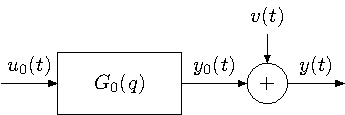
\includegraphics{\thisDir/figs/tikz0.pdf}
\caption{SISO LTI discrete-time system in an output error setup.}
\label{lpmtdrep}
\end{figure}

Numerous parametric identification techniques are devoted to the development of parametric plants $G(q,\theta)$ and parametric noise models  $H(q,\theta)$, where  $\theta$ is the model parameters vector  \citep{Ljung1999,Soderstrom1989}.

In this paper, however, a nonparametric technique is developed, %the identification problem is
formulated in the frequency domain, consistent with \citep{Pintelon2012,Mahata2006}. The following  choices are made:

\begin{itemize}

\item

The work in this paper is for discrete-time systems. Denote the $k^{th}$ discretized frequency as $\Omega_k$ = $e^{-j2{\pi}kf_s/N}$, with $f_s$ the sample frequency and $N$ the total number of sample points.
\item

Describe the parametric plant model  $G(q,\theta)$ by the nonparametric FRF counterpart  $G(\Omega_k)$  at the $k^{th}$ frequency.
\item

Describe  the parametric noise model $H(q,\theta)$ (associated with the output noise source $v(t)$) by a nonparametric noise variance contribution $\sigma^2_v(\Omega_k)$ at the $k^{th}$ frequency.

\end{itemize}

The rest of the paper is structured as follows. Section \ref{se:theoryLPMandWindowing} covers the theory on the LPM and windowing for an OE setup.
Section \ref{se:smoothingFRFestimate} discusses the novel smoothing method.



Ultimately, in \secref{se:simResults}, simulation results of the following FRF estimates and their corresponding variances are compared: (i) the smooth LPM estimate $\hat{G}_\text{sm-poly}(\Omega_k)$, (ii) the LPM estimate $\hat{G}_\text{poly}(\Omega_k)$.

These FRF estimates are also compared with the true \gls{LTI} system ${G}_0(\Omega_k)$.
Discussion of the simulation results is then followed by a conclusion in \secref{se:conclusion}.

\subsection{Theory on the LPM and Windowing: \glsentrytext{OE} Setup}
\label{se:theoryLPMandWindowing}

Details of the theory pertaining to this section may be found in \citep{Schoukens2009LPM}, basic aspects of which are presented below.


\subsubsection{Spectral Nonparametric Model and Assumptions}

Using convolution, the noiseless output signal in \figref{lpmtdrep} is $y_0(t) = g_0(t)*u_0(t)$, where the signals are sampled at $t = 0, 1, 2,...,N-1$ and the excitation signal $u_0(t)$ is random noise. As shown in \citep{Pintelon2012} and \citep{Pintelon1997} the \gls{DFT} spectra of the sampled signals at the frequency $\Omega_k$ are related as follows:
\begin{equation}\label{lpmleak}
Y_0(k)=G_0(\Omega_k)U_0(k)+T_G(\Omega_k)
\end{equation}
where $U_0(k)$ is the \gls{DFT} spectrum of the random noise excitation,  $G_0(\Omega_k)$ is the transfer function and $T_G(\Omega_k)$ is the transients leakage term.
In this paper, the \gls{DFT} of a signal $x(t)$ is defined explicitly as  \citep{Oppenheim1983}

\begin{equation}\label{eq:defDFT}
X(\Omega_k) = \frac{1}{\sqrt{N}}\sum_{t=0}^{N-1}x(t)e^{-\frac{j2\pi kt}{N}}
\end{equation}


The following assumptions are consistent with \citep{Schoukens2009LPM} for an OE setup (\figref{lpmtdrep}):
\begin{assumption}
The SISO system $G_0$ and  the transients leakage spectrum $T_G$ are both smooth functions of the frequency.
\end{assumption}



\begin{assumption}

The spectrum of the  input signal $U_0$ is not a smooth function of the frequency, but a rough function, for example $U_0(k+1) - U_0(k)$ should not vanish to zero. %i.e. $U_0(k+1) - U_0(k) \neq 0$.
\end{assumption}

In other words, for the excitation signal to be rough: the magnitude of the spectral difference $|U_0(k+1) - U_0(k)|$ must have a probability of 1 (unity) for it to remain in the same order of magnitude as $|U_0(k)|$, irrespective of the record length $N\rightarrow\infty$ and the corresponding  frequency resolution $f_0\rightarrow{0}$.


\begin{assumption}
The measured output signal is $y(t) = y_0(t) + v(t)$ with the exact input signal $u_0(t)$ known.
\end{assumption}


\begin{assumption}
The filtered white noise $v(t) = H_0(q)e(t)$ is the disturbing noise source at the output.
\end{assumption}


\subsubsection{The Hanning Window and the \glsentrytext{LPM}}\label{se:LPMFRFest}%\label{se:FRFhanningLPM}
\paragraph{Windowing}
The effect of windowing may be  exemplified by use of the Hanning window, which is very popular.
In a nutshell, the Hanning window is effective in reducing  the leakage errors, but  with a trade off of increased interpolation errors. %This is because the term $G_0(\Omega_k)U_0(k)$ in equation \eqref{lpmtd1} is not smooth and $G_0(\Omega_k)$ varies with the frequency.
Pertinent details of the Hanning window are discussed in \citep{Schoukens2006LPM,Antoni2007FRF,Schoukens2009LPM,Wellstead1981} and \citep{Harris1978}.

The anomalies due to interpolation errors, associated with windowing, can easily be mitigated or circumvented by use of the LPM. As shown in \citep{Pintelon2012}, the leakage errors are reduced from  $\mathcal{O}({N}^{-1})$, for Hanning windowing, to $\mathcal{O}({N}^{-3})$ or better, for the LPM.


\paragraph{Formulation of the Linear LS LPM}
The LPM is formulated as a nonparametric local-linear-least-squares (LS) estimate using the full data record of length $N$ as outlined below \citep{Schoukens2009LPM}.
\citet[Section 7.2.2]{Pintelon2012} gives the general formulation of the \gls{LPM} for \gls{MIMO} systems.
The formulation in this paper is a summary for a \gls{SISO} system.

The \gls{DFT} spectra at the output of the \gls{SISO} system in \figref{lpmtdrep} are derived from equations \eqref{lpmtd1} and \eqref{lpmleak}, \emph{viz}:
\begin{equation}\label{lpm1spectra}
Y(k)=G_0(\Omega_k)U_0(k)+T(\Omega_k)+V_0(k)
\end{equation}
where $V_0(k) = H_0(\Omega_k)E(k)$ is a noise term, and $T(\Omega_k)$ is the leakage term. The latter is the sum of the system and the noise leakage terms, i.e. $T(\Omega_k) = T_G(\Omega_k) + T_H(\Omega_k)$.

The smooth characteristics of $G_0(\Omega_k)$ and $T(\Omega_k)$ allow for the use of the Taylor series representations at the frequency lines $k+r$ in a frequency domain window of width $2n+1$, with a remainder $\mathcal{O}\left(\frac{r}{N}\right)^{(R+1)}$ of the first order Taylor series expansion \citep{Schoukens2009LPM}, \emph{viz}:
\TODO{ordos are incorrect: notation-wise}
\begin{align}\label{lpmGTaylorS}
G_0(\Omega_{k+r})&=G_0(\Omega_k)+\sum_{p=1}^{R}g_p(k)r^p+
\bigO{\left(\frac{r}{N}\right)^{(R+1)}},
\\
\label{lpmTTaylorS}
T(\Omega_{k+r})&=T(\Omega_k)+\sum_{p=1}^{R}t_p(k)r^p+N^{-1/2}
\bigO{  \left(\frac{r}{N}\right)^{(R+1)}  }
,
\\
\text{where}&\ r\in\mathbb{W}_n,\quad \mathbb{W}_n = \{-n,-n+1,\dots,n\}
\end{align}

The choice of the tunable parameters $n$ and $R$ is discussed later on.

Neglecting the remainder, the Taylor series approximation of \eqref{lpm1spectra} can be written in a matrix vector form, \emph{viz}:
\begin{equation}\label{lpmGTMatrix}
Y(k+r)\approx{K(k, r)\theta(k)+V_0(k+r)}
\end{equation}
where $\theta(k)\in\mathbb{C}^{2R+2}$ is the column vector of the  parameters ($G_0(\Omega_k)$, $T(\Omega_k)$, $g_p$, $t_p$, and $p = 1, 2, ...., R$) and $K(k, r)$ is the row vector of their respective coefficients:
\begin{align}
K(k,r) = &\left[
\begin{matrix}
U_0(k+r) & U_0(k+r)r & \dots
\end{matrix}
\right.
\\
&\quad\left.\begin{matrix}U_0(k+r)r^R & 1& r&\dots&r^R\end{matrix}\right]\nonumber
\end{align}


Equation \eqref{lpmGTMatrix} can be written in the more compact (stacked vectors) form:
\begin{equation}\label{lpmGTMatrixStack}
Y_n(k)\approx K_n(k)\theta(k)+V_n(k)
\end{equation}
where $Y_n(k), V_n(k)\in\mathbb{C}^{2n+1}$, and $K_n(k)\in\mathbb{C}^{(2n+1)\times(2R+2)}$ are the stacked values of $Y(k+r)$, $K(k,r)$, and $V_0(k+r)$, respectively, for $r\in\mathbb{W}_n$.
The estimates of the parameters $\theta(k)$ are obtained as the minimizers of the least squares problem, \emph{viz}:
\begin{align}\label{eq:LSsolutionLPM}
\hat\theta(k) = \argmin_{\theta(k)} \left\|Y_n(k) - K_n(k)\theta(k)\right\|_2^2
\end{align}

The formulation of equation \eqref{eq:LSsolutionLPM} must take into account the fact that  a full rank of $K_n$ requires $n \geq R + 1$. The choice $n = R + 1$ results in the highest variance on the estimate, but with the smallest interpolation error \citep{Schoukens2009LPM}. %(per JL)!


The values $R = 2$, and $n=R+1=3$ will be used in the \gls{LPM}.

When substituted into equations \eqref{lpmGTaylorS} and \eqref{lpmGTMatrix},  these yield the following quadratic local polynomials of $G_0$ and $T$ around a central frequency $\Omega_{k}$:
\begin{align}\label{lpmImplQuadG}
G_0(\Omega_{k+r})&\approx G_0(\Omega_k)+g_1r+g_2r^2
\\
T(\Omega_{k+r})&\approx T(\Omega_k)+t_1r+t_2r^2\label{lpmImplQuadT}
\end{align}

\noindent
($r\in\mathbb{W}_3$)
and the vector of parameters:

\begin{equation}\label{lpmThetaEst}
\theta^\top(k)=\left[G_0(\Omega_k) \ g_1 \ g_2\  T_G(k)\  t_1 \ t_2\right]
\end{equation}
The \gls{LPM} estimate of the FRF is the first element of the estimate $\hat\theta(k)$, obtained from \eqref{eq:LSsolutionLPM}, \emph{viz}:
\begin{equation}
\hat{G}_\text{poly}(\Omega_k) = \hat\theta_1(k)
\end{equation}


The estimation of $\hat{G}_\text{poly}(\Omega_k)$ at a single frequency $\Omega_k = 0.586$~Hz is illustrated in \figref{LPM_Schematic_EG}.% centered at $k$, where $r = 0$.
\begin{figure}[htb] %  figure placement: here, top, bottom, or page
   \centering
   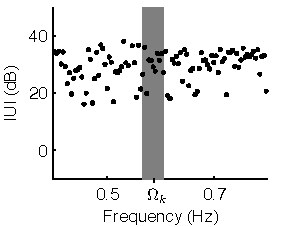
\includegraphics[scale=0.92]{\thisDir/figs/spectUOmegak}
   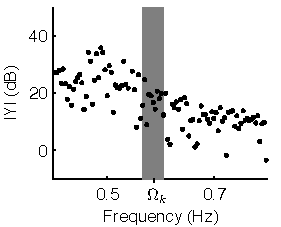
\includegraphics[scale=0.92]{\thisDir/figs/spectYOmegak}
   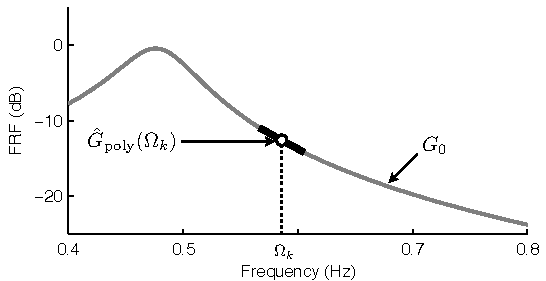
\includegraphics{\thisDir/figs/LPMfigOmegak}
   \caption{Illustration of the \gls{LPM}. Top figures: input spectrum (left) and output spectrum (right). A small band is selected (gray area, top figure), in which $\hat G_\mathrm{poly}(\Omega_{k+r})$ is estimated (black thick line, bottom figure) as a local polynomial. Only its central value $\hat G_\mathrm{poly}(\Omega_k)$ (white circle) is retained. This procedure is repeated for all $\Omega_k$.}
   \label{LPM_Schematic_EG}
\end{figure}
This procedure is repeated at each central frequency $\Omega_k$ for  $k\in \{1,\dots,N/2\}$ (i.e. the entire frequency band, including Nyquist, but excluding DC, and regularizing at the boundaries). This completes the \gls{LPM}, yielding an intrinsic averaging of the spectra of the estimated \gls{FRF}, $\hat{G}_\text{poly}(\Omega_k)$.

\section{Smoothing the \gls{FRF} estimate}\label{se:smoothingFRFestimate}
The method for smoothing (improving) the \gls{LPM} estimate of the frequency response function  is presented in this section together with pertinent assumptions. After obtaining the \gls{LPM} estimate of the \gls{FRF} (denoted as $\hat{G}_{\mathrm{poly}}(\Omega_k)$) from \secref{se:LPMFRFest}, the smoothing method is decomposed into the following procedures, which will be elaborated on later:
\begin{enumerate}
\item The impulse response $\hat g_\mathrm{poly}(t)$  is computed from the \gls{IDFT} of $\hat{G}_{\mathrm{poly}}(\Omega_k)$.

\item
Assuming that the impulse response decays exponentially in time, the noise is bound to predominate after a certain time interval.

\item
An accurate estimate of the \gls{DC} value of the \gls{FRF} is computed by inspecting the average value of the tail of the estimated impulse response.

\item
A truncation is effected at the point beyond which the data record (impulse response) is buried in noise.

This action results in smoothing the \gls{LPM} estimate of the \gls{FRF}.
An exponential fitting method is introduced to determine the truncation point.
\end{enumerate}

These procedures require that the following assumptions are satisfied.

\begin{assumption}
The estimate $\hat G_\mathrm{poly}(\Omega_k)$ is available at all frequencies $\Omega_k$ for $k\in\{1,2,\dots,N/2\}$.
\end{assumption}

This assumption ensures that the impulse response corresponding to the \gls{FRF} can be computed (up to its mean value). It requires that the input signal excites the whole unit circle. This is satisfied, for instance, by using white noise as an excitation signal.


\begin{assumption}\label{ass:imprespdecay}
The impulse response $g(t)$ decays exponentially over time, i.e. $\exists A \in \PositiveRealNumbers, \exists a \in \NegativeRealNumbers \without \Set{0}, \forall t \in \PositiveRealNumbers: \abs{g(t)} \leq A \exp(- a t)$.
\end{assumption}

\begin{assumption}\label{ass:decay90perctime}
Within $90\%$ of the measurement window, the impulse response decays
 to a level that is indistinguishable from the noise.
\end{assumption}

Note that Assumptions \ref{ass:imprespdecay} and \ref{ass:decay90perctime} exclude the possibility of considering a system that is a pure integrator.

\subsubsection{Obtaining the Impulse Response Function}

The estimated impulse response function  $\hat g_{\mathrm{poly}\setminus \mathrm{DC
}}(t)$ is obtained explicitly via the \gls{IDFT} of the \gls{LPM}-estimate $\hat G_\mathrm{poly}(\Omega_k)$ of the \gls{FRF} in accordance with equation \eqref{eq:defDFT}, \emph{viz}:

\begin{align}\label{eq:impRespiDFT}
\hat g_{\mathrm{poly}\setminus \mathrm{DC
}}(t) &= \frac{1}{\sqrt{N}}\sum_{k=1}^{N-1}\hat G_\mathrm{poly}(\Omega_k)e^{\frac{j2\pi kt}{N}}
\end{align}
where the estimated \gls{FRF} in the frequency band between  the Nyquist and the sample frequencies is obtained as follows:

\begin{align}
\hat G_\mathrm{poly}(\Omega_{N-k}) = \overline{\hat G_\mathrm{poly}(\Omega_k)},\ \text{for}\ k=1,\dots,N/2
\end{align}
(with $\conj{\hat G_\mathrm{poly}}$ the complex conjugate of $\hat G_\mathrm{poly}$) to ensure $\hat g_\mathrm{poly}(t)$ to be real.

\TODO{fix reference Section II}
Smoothing of the estimated \gls{FRF} requires the correct estimate of the impulse response. Unfortunately, the \gls{LPM} presented in \secref{se:theoryLPMandWindowing} and in \citep{Schoukens2009LPM} does not estimate the \gls{FRF}  at the frequency $\Omega_0$ (i.e. \gls{DC} value of the \gls{FRF}), hence the subscript $\setminus\mathrm{DC}$ in equation \eqref{eq:impRespiDFT}. Consequently, the mean value of the corresponding estimated impulse response given in equation \eqref{eq:impRespiDFT} is not correct. 
This limitation is lifted by developing a simple estimator of the mean value, presented below.

\subsubsection{Estimating the \glsentrytext{DC} Value of the \glsentrytext{FRF}}\label{se:DCvalueEst}
The correct mean value of the impulse response accounts for (i.e. estimates) the \gls{DC} value of the \gls{FRF}. A time-domain method is proposed for estimating the mean value of the impulse response in equation \eqref{eq:impRespiDFT}. %The first is a frequency-domain technique and the second is a time-domain technique.

According to Assumption~\ref{ass:imprespdecay}, the true impulse response tends to zero asymptotically; and by Assumption~\ref{ass:decay90perctime}, the last $10\%$ of the estimated impulse response is noise, plus a constant value due to an inaccuracy in the average value of the impulse response. The correct estimate of the mean value is obtained by shifting the whole signal such that the last $10\%$ of the impulse response is centered around 0.
To this end, the following procedure is executed:


\begin{enumerate}
\item Compute the mean value $m_{g10}$ of the last 10\% of the impulse response $\hat g_{\mathrm{poly}\setminus \mathrm{DC
}}(t)$, estimated by the \gls{LPM}, as %$\hat g_\mathrm{poly}(t)$ as
\begin{align}
m_{g10} = \frac{1}{\lceil0.1N - 1\rceil}\sum_{t=\lfloor0.9N\rfloor}^{N-1}\hat g_{\mathrm{poly}\setminus \mathrm{DC
}}(t)
\end{align}

\item Next, subtract the computed mean value $m_{g10}$ from $\hat g_{\mathrm{poly}\setminus \mathrm{DC
}}(t)$ to obtain the improved impulse response $\hat g_\mathrm{poly}(t)$, \emph{viz}:


\begin{align}
\hat g_\mathrm{poly}(t) = \hat g_{\mathrm{poly}\setminus \mathrm{DC
}}(t) - m_{g10},\ \text{for}\ t=0,1,\dots,N-1
\end{align}


\end{enumerate}

\subsection{Truncation of the Impulse Response Via Exponential Fitting}\label{se:truncImpulseResp}

The \gls{FRF} estimate is smoothed by truncating the estimated impulse response function. The truncation is applied at the time index beyond which the signal is indistinguishable from the noise.

This is done via the fit of an exponential function on the maxima of the impulse response, implemented as follows.

\begin{enumerate}
\item Obtain the estimate of the impulse response $\hat g_\mathrm{poly}(t)$ from the LPM, corrected for its DC value as discussed in Section \ref{se:DCvalueEst}. Henceforth, $\hat g_\mathrm{poly}(t)$ will simply be denoted as $\hat g(t)$. %In the remainder of this procedure description $\hat g_\mathrm{poly}(t)$ will be simply denoted $\hat g(t)$.

\item Obtain an estimate $\hat \sigma_\mathrm{n}$ of the standard deviation of the noise from the last 10\% of the data, \emph{viz}:

\begin{align}
\hat \sigma^2_\mathrm{n}=\frac{1}{\lceil0.1N - 1\rceil}\sum_{t=\lfloor0.9N\rfloor}^{N-1}\hat g^2(t).
\end{align}
This is valid, as per Assumption \ref{ass:decay90perctime}.

%This assumes that the impulse response of the system is not longer than 90\% of the length of the measured time interval.

\item Obtain $\mathbb{T}_\mathrm{HSNR}$ as the set of time instants where $\hat g(t)$ is significantly above the standard deviation of the noise. Only samples with absolute values of at least $5\hat\sigma_\mathrm{n}$ are retained: %Only samples with an absolute value of at least $5\hat\sigma_\mathrm{n}$ have been retained:
\begin{align}
\mathbb{T}_\mathrm{HSNR} = \left\{
t:|\hat g(t)|\geqslant 5\hat\sigma_\mathrm{n}
\right\}.
\end{align}

\noindent
(Subscript HSNR stands for High \gls{SNR}.)

%This choice leaves a probability of $6\times10^{-7}$ of retaining a pure noise sample, in the case of Gaussian noise.

\item Find the set $\mathbb{T}_\mathrm{max}$ of indices corresponding to monotonically decreasing maxima of the impulse response:
\begin{align}\label{eq:TmaxDef}
\mathbb{T}_\mathrm{max} = \left\{
t: \left| \hat g(t)\right|>
\left|\hat g(t')\right|,
t < t' < N \land t'\in\mathbb{T}_\mathrm{HSNR}
\right\},
\end{align}

\item Fit an exponential function $Ae^{at}$ approximating $\hat g(t)$, in $t_\mathrm{max}\in\mathbb{T}_\mathrm{max}$. This is done by solving the following expression

\begin{align}\label{eq:expFit}
\ln \left|\hat g(t)\right|\approx \ln A+at,\ \mathrm{with}\ t\in\mathbb{T}_\mathrm{max},
\end{align}
for $\ln A$ and $a$ in a least squares sense.
This is a quadratic problem in the parameters and, thus, amount to a convex optimization problem that can be solved directly.
Since  $\ln \left|\hat g(t)\right|$ decreases for an increasing $t$ in $\mathbb{T}_\mathrm{max}$ (by construction in equation \eqref{eq:TmaxDef}), the estimated $a$ from equation \eqref{eq:expFit} is always negative.

\item
Determine the first time-instant $t_\mathrm{trunc}$ at which the estimated exponential gets significantly below the noise floor, \emph{viz}:

\begin{align}\label{eq:truncTimeExpFit}
t_\mathrm{trunc} = \min \left\{t:Ae^{at} < \gamma\hat\sigma_\mathrm{n}\right\}
\end{align}

\noindent
where the parameter $\gamma$ can be tuned such that an appropriate trade-off between the decreased variance and the increased bias on the estimated smoothed FRF is found. This is discussed below. %(see the discussion below).
% The value of $\gamma$ to be used depends on the system. %$\gamma = 0.1$ was found to be a good rule of thumb.

\item
 Truncate the estimated impulse response for $t \geqslant t_\mathrm{trunc}$.

\end{enumerate}

\begin{figure}[tbh] %top bottom here
\centering

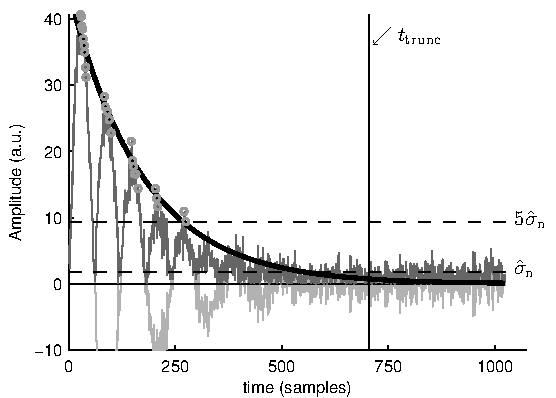
\includegraphics[scale=0.9]{\thisDir/figs/expFitest}
\caption{Truncation of the impulse response via the fit of  an exponential. The light gray line is the noisy impulse response, and the dark gray one is its absolute value. Gray circles: monotonously decreasing maxima, greater than $5\hat\sigma$, as per \eqref{eq:TmaxDef}. Black thick line: estimated exponential function \eqref{eq:expFit}.}
\label{FRF_truncate_expfitter}
\end{figure}

As an illustration, this procedure was applied to the noisy impulse response of the system described by the following difference equation:

\begin{equation}
y_0(t) = 2.583y_0(t - 1) -2.176y_0(t - 2)+0.592y_0(t-3) + u(t)
\end{equation}

The measured signal was disturbed by random white noise, $y(t) = y_0(t) + e(t)$, such that the \gls{SNR} was $14.2\unit{dB}$.
The result is depicted in \figref{FRF_truncate_expfitter}. An exponential function (black thick line) is fitted on the maxima (gray circles) of the absolute value of a noisy impulse response (dark gray line). The truncation time (black vertical line) $t_\mathrm{trunc}$ was selected as the time instant at which the fitted exponential fell below $0.4\hat\sigma_n$ (i.e. $\gamma = 0.4$ in equation \eqref{eq:truncTimeExpFit}).

\paragraph*{Considerations on the choice of $\gamma$}

\begin{itemize}
\item The tuning parameter $\gamma$ is application- and system-dependent.  A higher value lowers the variance of the estimated \gls{FRF}, but increases its bias, and vice versa.

\item
The bias error is highest in the vicinity of (sharp) resonance peaks. If the latter is to be estimated with a high accuracy, a value $\gamma \ll 1$ must be used. %If the latter must be estimated with a high accuracy, a value $\gamma \ll 1$ must be preferred.

\item If one is interested in obtaining a smooth initial estimate of the \gls{FRF}, a (small) bias error is acceptable, and choosing $\gamma \approx 1$ was found to be a good rule of thumb.
\end{itemize}

\subsection{Simulation Results}\label{se:simResults}

\figref{figLPMvsTrunc} and \figref{fig:pdfAndRMSeVStruncTime} compare the \gls{LPM} with and without truncation of the impulse response.
They were obtained from simulations on  the system described by the following simulation equations, which are relevant to the \gls{LPM} outlined in \secref{se:LPMFRFest}:
\begin{subequations}
\label{eq:systemSimulations}
\begin{align}
y_0(t)  &= 1.5371y_0(t-1)    -0.9025y_0(t-2) + u(t)
\\
y(t) &= y_0(t) + e(t),
\end{align}
\end{subequations}
where $e(t)$ is a white noise sequence, such that the \gls{SNR} of the output signal is $18.3\unit{dB}$.


\begin{figure}[tbh] %top bottom here
\centering


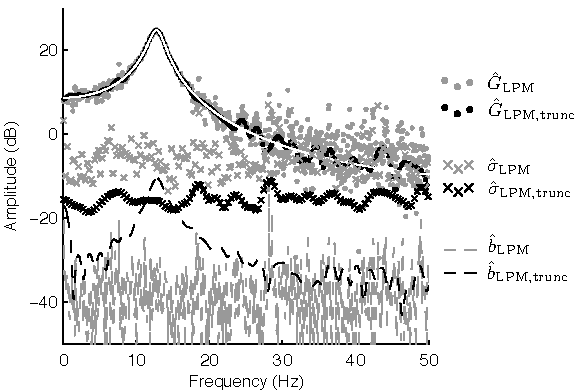
\includegraphics[scale=0.9]{\thisDir/figs/figLPMvsTruncWlegend}

\caption{Comparison of the \gls{LPM} and Truncated \gls{LPM} estimates of the \gls{FRF} for an \gls{SNR} of $18.3\unit{dB}$. The gray plots pertain to the \gls{LPM} estimate without truncation, the black ones to the \gls{LPM} with truncation (trunc). Dots: \gls{FRF} estimates $\hat{G}$. Crosses: sample standard deviations $\hat{\sigma}$. Dashed lines: bias $\hat{b}$. White line: the true system $G_0$.}
\label{figLPMvsTrunc}
\end{figure}





In \figref{figLPMvsTrunc} one observes the following:
\begin{itemize}
\item
a decrease of the variance on the truncated estimate of about $10 \unit{dB}$,  i.e. a decrease of the black crosses, compared to the gray ones, is observed. %i.e. a decrease of the black crosses w.r.t.~the gray ones is observed.

\item
the error on the truncated \gls{LPM} estimate is strongly correlated over the frequency. This must be taken into account when formulating a maximum likelihood parametric estimator of the system.

\item
an increase of the bias of the truncated estimate, especially in the vicinity of the resonance frequency. Still, this bias lies below the variance of the non-truncated estimate. As such, for a single experiment, the increase in bias still yields a better estimate when truncation is invoked.

This bias depends on the time instant at which the truncation is performed, as discussed below.

\end{itemize}

\begin{figure}[htb] %  figure placement: here, top, bottom, or page
   \centering



	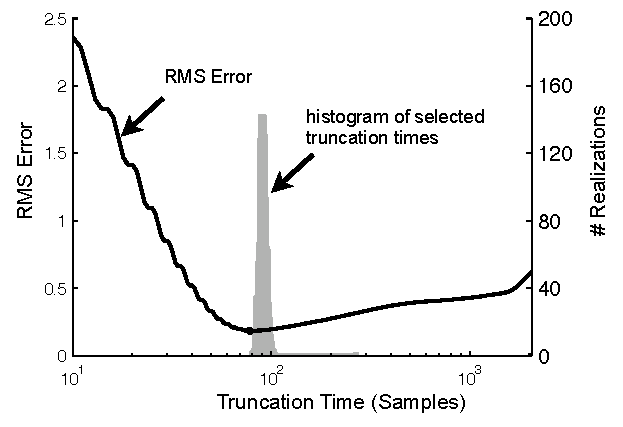
\includegraphics{\thisDir/figs/HistogramExpFitting.pdf}
 \caption{Black full line (left hand side y-axis (ordinate)): total \gls{RMS} error as a function of the truncation time (the single black dot is the minimum of the \gls{RMS}). Gray histogram (right hand side y-axis (ordinate)): selected truncation times for 1000 noise realizations by the exponential fitting methods.}



   \label{fig:pdfAndRMSeVStruncTime}
\end{figure}

In \figref{fig:pdfAndRMSeVStruncTime}, the black graph is the \gls{RMS} error of the estimated \gls{FRF} (without the \gls{DC} value) as a function of the time $t_\mathrm{trunc}$ at which the impulse response is truncated. Its minimum is indicated by a black dot, to the left of which a steep increase is observed. This is due to a bias error. To the right hand side of the minimum, the \gls{RMS} error increases very gradually, due to an increase of the noise variance.

A good practice would be to truncate the impulse response at the minimizer (black dot) of the \gls{RMS} error. However, it should be noted that this minimizer is unknown in practice, because it would require
the true \gls{FRF}.

The truncation time is determined from the data as described in Section \ref{se:truncImpulseResp}. This was done on $1000$ realizations of the noise, and depicted in \figref{fig:pdfAndRMSeVStruncTime} by the histogram.
Clearly, the method for selecting the truncation time $t_{\mathrm{trunc}}$ has a good overall performance, based on the mode of its distribution. A closely grouped set of values for $t_{\mathrm{trunc}}$ is obtained around the $90^{\text{th}}$ sample, without significant outliers.


From the plot, we can conclude that the \gls{RMSE} increases rapidly when $t_{\mathrm{trunc}}$ is smaller than the optimal.
On the other hand, selection of a value of $t_{\mathrm{trunc}}$ that is too large, is not nearly as detrimental to the modeling error.
The graph also shows that the \gls{RMSE} of the model can be decreased from $0.62$ (without truncation) to $0.18$ when the optimal truncation is applied. Also, one observes a low sensitivity of the \gls{RMSE} w.r.t.~$t_\mathrm{trunc}$, when truncating at times beyond that optimum. Therefore, a somewhat conservative truncation method is still likely to yield a close to optimal result.

\subsection{Conclusion}\label{se:conclusion}

The paper introduced a novel time domain method to smooth the \gls{LPM}-estimate of an \gls{FRF}. It consisted of, after obtaining the \gls{FRF} from the \gls{LPM}, computing the associated estimated impulse response via the \gls{IDFT}.
Then, it was determined statistically at which time index the impulse response had decayed below the noise floor, yielding a point beyond which the response may be set to zero.

The results clearly indicate that the truncation technique lowers the impact of the noise on the estimate of the \gls{FRF}, resulting in a decreased variance. A bias-variance trade-off is possible by tuning the time beyond which the impulse response is indistinguishable from the noise.


% \bibliographystyle{IEEEtran}
% \bibliography{MikayaBibliography}
% \end{document}
